\section{Decorator}

O padrão Decorator permite adicionar responsabilidades a um 
objeto de forma dinâmica. Essa dinamicidade é alcançada 
substituindo a herança por uma agregação, permitindo que a 
classe decorada delegue responsabilidades para as classes que 
a extendem. As classes de extensão implementam uma mesma 
interface que as classes decoradas e possuem um objeto dessa 
mesma classe entre seus atributos. Dessa forma, uma classe 
de extensão pode tanto referenciar outra classe de extensão 
quanto o objeto decorado, formando uma estrutura de pilha 
onde o elemento ao fundo é o objeto decorado que será o 
alvo das operações de todos os extensores presentes na 
estrutura.

O maior problema resolvido pelo Decorator é a grande 
quantidade de classes que deveriam existir caso houvessem 
muitas extensões para uma classe. O problema cresce ainda 
mais quando é necessário que essas funcionalidades mudem 
dinamicamente, gerando diversas combinações de grupos de 
funcionalidades possíveis.

\begin{figure}[htb]
	\caption{\label{fig_grafico}Estrutura do Decorator}
	\begin{center}
	    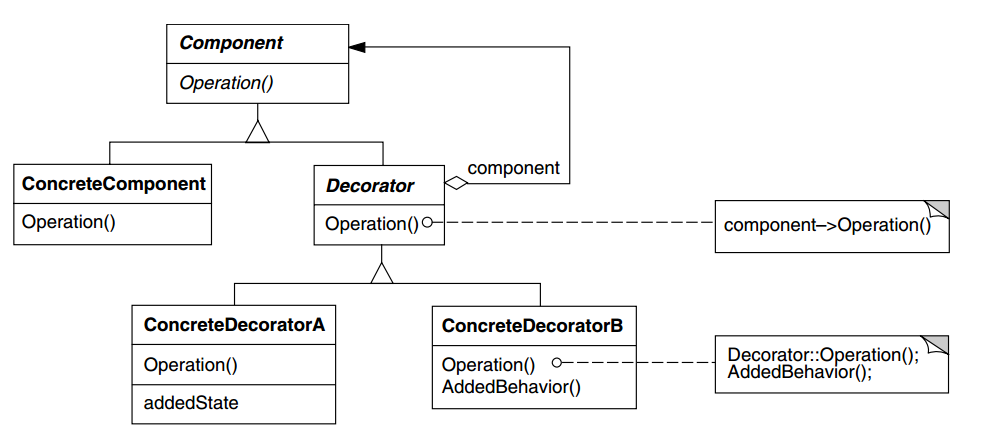
\includegraphics[scale=0.5]{5_padroes-contexto-funcional/5.2_estruturais/5.2.4_decorator/diagram.png}
	\end{center}
\end{figure}

Exemplo Orientado a Objetos:

\begin{lstlisting}[caption={Decorator Orientado a Objetos},label=oodecorator]



\end{lstlisting}

Contexto Funcional:

O mesmo objetivo é alcançado de forma simples através de 
composição de funções. Caso um valor precise ser decorado 
com diversas funções, uma função recebe esse valor como 
parâmetro e uma lista com todas as funcionalidades que irão 
estendê-lo. Essas funções são então chamadas uma por uma, 
gerando também uma pilha de chamadas que finalmente 
retorna o resultado da combinação de todas as operações.

\begin{lstlisting}[caption={Decorator Funcional},label=fpdecorator]
    

    
\end{lstlisting}